\chapter{Technologieën}
\label{ch:technologystack}
In dit hoofdstuk wordt er gekeken naar technologieën die eventueel toepasbaar zijn op het ontwikkelproces van de nieuwe editor. Eerst zullen de huidige gebruikte technologieën op een rijtje worden gezet. Hierna zal er gekeken worden naar de toekomst van de editors. Tenslotte zal het probleem in kaart worden gebracht waarop eventuele oplossingen zullen worden geadviseerd.

\section{Technology stack}
Onder een ‘technology stack’ (of ‘tech stack’) verstaan we de onderliggende bouwblokken waarop de desbetreffende applicatie gebouwd is. Deze bouwblokken bestaan uit onder andere frameworks, libraries, programmeertalen, softwareproducten en eventuele tooling\cite{BlogTechStack}.

\subsection{Waarom is dit belangrijk?}
Het is erg belangrijk om de tech stack in kaart te brengen omdat er elementaire informatie uit te halen is. De tech stack geeft inzicht in hoe het huidige product in elkaar steekt en eventuele consequenties wanneer er componenten in de stack aangepast worden. Dit is noodzakelijk voor het maken van een nieuwe editor die geïntegreerd moeten worden in een al bestaande tech stack. Door deze stap te nemen wordt er goed gekeken naar hoe de nieuwe editor in het totaal plaatje zou kunnen passen. Zo kan het voor komen dat er bepaalde software wordt gebruikt die nauw samenwerkt met de huidige editors. Dit heeft als gevolg dat de nieuwe editors deze samenwerking moeten ondersteunen.

\pagebreak
\section{De technology stack van \&ranj}
Om de ontwikkeling van narrative games te ondersteunen heeft het bedrijf een ontwikkelomgeving opgezet. Het doel van deze omgeving is om het ontwikkelingsproces inzichtelijk te maken voor verschillende disciplines en overtollig werk, zoals het opzetten van een nieuw project, te vermijden door een leeg raamwerk aan te bieden. Dit raamwerk bevat templates (het NGT), editors en programma’s om de efficiëntie en collaboratie tijdens het ontwikkelproces te bevorderen.

De ontwikkelomgeving voor narrative games heeft een onderliggende tech stack die bestaat uit verschillende programmeertalen, libraries, frameworks, Integrated development environments (IDE’s) en externe applicaties. Stackshare.io\footnote{https://stackshare.io/} een website waar stacks van (bekende) bedrijven kunnen worden ingezien, deelt deze op in de volgende lagen\cite{StackShareCategories}:

\begin{itemize}
    \item \textbf{Application and Data}, dit betreft onder andere programmeertalen, frameworks \& libraries.
    \item \textbf{Utilities}, hieronder vallen analytics en eventuele hulpmiddelen.
    \item \textbf{DevOps}, gaat over de build, test, deploy processen en het monitoren van het product.
    \item \textbf{Business Tools}, omvangt bestaande oplossingen voor samenwerking en marketing.
\end{itemize}

De onderliggende tech stack die de ontwikkelomgeving van narrative games ondersteund kan uiteen worden gezet volgens deze lagen. Hierdoor kan inzicht worden verkregen in hoe de huidige ontwikkelomgeving in elkaar steekt. Het bedrijf beschrijft de narrative game: ‘Mission Zhobia: Winning the Peace’ als een typische narrative game. Dit spel beschikt over een tech stack zoals uiteengezet in \autoref{tab:currentechstack}.

\begin{table}[htb]
    \centering
    \begin{tabular}{ | l | l | }
        \hline
        \multicolumn{2}{|c|}{\textbf{Narrative game - Technology stack}} \\
        \hline
        \multicolumn{2}{|c|}{Application and Data} \\
        \hline
        \&ranj JavaScript software library & \tabitem Javascript(ECMAScript5) \\
        & \tabitem CreateJS suite \\
        \hline
        Narrative game template & \tabitem Javascript(ECMAScript5) \\
        & \tabitem CreateJS suite \\
        & \tabitem SomaJS \\
        \hline
        \&ranj ActionScript3 software library\footnote{Bestaat uit 3 ActionScript3 libraries gemaakt door \&ranj, maar heeft één verzamelnaam} & \tabitem ActionScript3 \\
        \hline
        Story- \& dialog editor & \tabitem ActionScript3 \\
        & \tabitem Apache Flex \\
        & \tabitem Flex wires \\
        \hline
        \multicolumn{2}{|c|}{Utilities} \\
        \hline
        Analytics & \tabitem Google Analytics \\
        \hline
        \multicolumn{2}{|c|}{DevOps} \\
        \hline
        Source control & \tabitem Beanstalk \\
        & \tabitem SourceTree \\
        \hline
        Deployment & \tabitem Jenkins \\
        & \tabitem SourceTree \\
        \hline
        IDE'S & \tabitem Adobe Flashbuilder\footnote{Bouwt ook de editors} \\
        & \tabitem Netbeans \\
        \hline
        Monitoring & \tabitem Pingdom \\
        \hline
        \multicolumn{2}{|c|}{Business Tools} \\
        \hline
        Collaboratie & \tabitem Trello \\
        & \tabitem G Suite \\        
        & \tabitem Slack \\
        \hline
        Documentatie & \tabitem \&ranj wiki \\
        \hline
    \end{tabular}
    \caption{Huidige technology stack}
    \label{tab:currentechstack}
\end{table}

Dit onderzoek betreft het opzetten van (flexibele) editors, daarom is het essentieel om de relatie tussen de huidige editors en de andere componenten binnen de ‘Application and Data’ laag in kaart te brengen. Hier kunnen eventuele risico’s/ consequenties naar aanleiding van veranderingen worden uitgelicht. Het is van belang dat de nieuwe editor goed aansluit bij de rest van de stack, zodat er onderbouwd advies op het gebied van veranderingen in de tech stack uitgebracht kan worden. De relaties tussen de componenten in de ‘Application and Data’ laag zijn weergeven in \autoref{fig:editorrelations}.

\begin{figure}[htb]
    \centering
    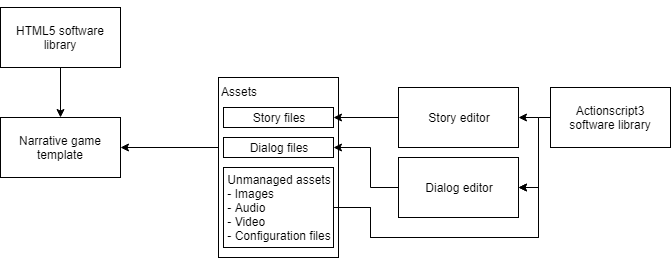
\includegraphics[width=0.75\textwidth]{StoryDialogEditorRelations}
    \caption{Story- en dialog editor relaties}
    \label{fig:editorrelations}
\end{figure}

\pagebreak
\section{Toekomst plannen}
\label{sec:editorfuture}
De toekomst van de editors zal, zoals in de inleiding beschreven, bestaan uit een web omgeving waarin meerdere personen tegelijk kunnen werken (collaborative editing). Hierin worden aanpassingen direct getoond aan teamleden wat het mogelijk maakt om met elkaar samen te werken aan dezelfde bestanden. Deze feature wordt nog interessanter wanneer klanten bij het ontwikkelproces betrokken worden. Zij zouden dan directe feedback of zelfs aanpassingen kunnen doen aan de game content. Het bedrijf geeft aan dat ze hier in de toekomst naar toe gaan werken, maar dat er meer onderzoek en resources nodig zijn om dit mogelijk te maken.

Hoewel dit vraagstuk niet in dit onderzoek past kan er wel rekening mee worden gehouden. Ook al zal het bedrijf voorlopig gebruik maken van een desktopapplicatie, moet er wel een blik op de toekomst geworpen worden. Bij het opzetten van een nieuwe editor vindt \organisation{} toekomstgerichtheid een belangrijk aspect; het bedrijf wil dan ook niet opnieuw een hele editor opzetten. Bij de keuzes die invloed hebben op de tech stack zal hier dan ook op worden gelet.

\pagebreak
\section{Pijnpunten in de huidige technology stack}
Beschikken over een stabiele en toekomstig gerichte tech stack is cruciaal voor een succesvol product. De tech stack heeft een directe invloed op de toegankelijkheid, schaalbaarheid en toekomstgerichtheid van de toekomstige editor. 

\subsection{Onzekerheid in de toekomst}
De huidige editors zijn gemaakt in Apache Flex. Dit is een omgeving waarin applicaties gemaakt kunnen worden met de hulp van ActionScript3 om logica te kunnen programmeren en MXML wat het definiëren van lay-outs toelaat in een XML-formaat\cite{WhatIsApacheFlex}. Projecten kunnen gecompileerd worden naar SWF-bestanden die kunnen worden uitgevoerd in een Flash- of Air run time. Vorig jaar, 25 juli, liet Adobe in een blog post weten dat ze ondersteuning voor Flash gaan beëindigen in 2020\cite{AdobeFlashFuture}. Hiernaast lijken er ook weinig updates plaats te vinden. Volgens de website van Apache Flex was de laatste update op 22 november 2017\cite{ApacheFlex}. Tenslotte werd Flash al eerder in meerdere populaire browsers standaard geblokkeerd vanwege veiligheidsredenen\cite{FlashWillBeBlocked}. Dit gaat tegen het toekomstbeeld van de editors in, het bedrijf wilt toewerken naar een webapplicatie. Verder leidt dit alles naar een onzekere toekomst van Apache Flex.

\subsection{Kleine community}
Het aanbod van libraries, klare oplossingen op veelvoorkomende problemen, is naar verhouding vrij minimaal omdat de community rond Apache Flex en ActionScript3 in vergelijking tot andere ontwikkelomgevingen relatief klein is. In de ‘populaire technologieën’ sectie van de enquête die Stack Overflow jaarlijks afneemt zijn Apache Flex en ActionScript3 niet te vinden\cite{StackOverflowSurvey2018}. Ondanks dat de Apache Flex community wel op Stack Overflow zit\cite{StackOverflowFlexQuestions}. Een kleinere community kan leiden tot minder hulp en een gebrek aan oplossingen voor veel voorkomende problemen. Dit is ook terug te zien aan ‘Flex Wires’, een library die de editors gebruiken om de nodes met lijnen aan elkaar te verbinden. De library is slecht aanpasbaar en biedt weinig functionaliteit. Verbindingen kunnen niet aangepast worden, er verschijnt altijd een grijze kromme lijn. Dit heeft als gevolg dat bepaalde features niet haalbaar zijn in de huidige editors. Hiernaast zitten er fouten in Flex Wires die alleen opgelost kunnen worden in de library zelf. Zo kunnen de verbindingen uit het niks verdwijnen, waardoor niet meer te zien is welke relaties er bestaan tussen nodes.

\subsection{Overtollige libraries}
Zowel de editors als het NGT maken gebruik van de \organisation{} software library welke generieke functionaliteiten en datastructuren bevat (zie \autoref{fig:editorrelations}). Echter moeten er twee libraries onderhouden worden omdat de huidige editors en het NGT geschreven zijn in verschillende programmeertalen. Het implementeren van nieuwe generieke functionaliteiten moet dubbel gedaan worden en de libraries moeten beide up-to-date zijn, omdat het NGT en de editors anders mogelijk niet meer goed samen kunnen werken.

\pagebreak
\section{Ontwikkelplatformen}
Het huidige ontwikkelplatform, Apache Flex, heeft een onzekere toekomst en sluit niet aan bij het toekomstbeeld van de editors die het bedrijf heeft. Het prototypen in een ontwikkelomgeving die die gericht op de toekomst is heeft meer waarde voor dit onderzoek.

\subsection{Aandachtspunten}
Bij het zoeken naar een gepast ontwikkelplatform werd er gelet op: de community om het platform heen, de toekomstgerichtheid van het platform en hoeveel werk het gaat kosten om deze te integreren in de huidige tech stack. Deze aspecten zijn gesorteerd op belang van hoog naar laag en worden hieronder vermeld met concrete vragen:

\begin{enumerate}
    \item Community
    \begin{itemize}
        \item Bestaat er een actieve community waarin mensen elkaar verder helpen met problemen?
        \item Zijn er bestaande oplossingen voor een visual scripting interface?
    \end{itemize}    
    \item Toekomstgerichtheid
    \begin{itemize}
        \item Door wie wordt het ontwikkelplatform onderhouden?
        \item Hoe ziet de toekomst van het ontwikkelplatform eruit?
        \item Kan er naast een desktopapplicatie ook uitgerold worden naar een web omgeving?
    \end{itemize}
    \item Integratie
    \begin{itemize}
        \item Sluit het ontwikkelplatform aan bij de rest van de tech stack?
        \item Sluit het ontwikkelplatform aan bij het bedrijf? Kunnen programmeurs overweg met het platform, zo niet hoe stijl is de leercurve?
    \end{itemize}
\end{enumerate}

\subsection{Selectie}
Er is een selectie gemaakt uit populaire en mogelijk passende ontwikkelplatformen:
\begin{enumerate}
    \item Haxe
    \item Electron
    \item NW
    \item Qt    
\end{enumerate}

\noindent Verder zullen de volgende ontwikkelplatformen kort worden behandeld, omdat deze potentie hadden maar al gauw niet de oplossing bleken te zijn.
\begin{enumerate}
    \item Unity
    \item Apache FlexJS
\end{enumerate}

\pagebreak
\subsubsection{Unity}
Het bedrijf wilt gebruik gaan maken van Unity voor de ontwikkeling van narrative games. Unity biedt een platform waarmee de verschillende disciplines in een projectteam beter samen kunnen werken. Het integreren van de nieuwe editor met Unity kan voordelen met zich meebrengen, zoals beter feedback en een betere workflow.
Echter is het niet aan te raden om een gehele editor in Unity te maken. Unity is van origine een game engine. Er kunnen simpele extensies gemaakt worden die getoond kunnen worden in Unity, maar een gehele narrative editor maken als Unity extensies vereist veel tijd. Hiernaast moeten extensies gemaakt worden op een manier die Unity afdwingt. Naast dat dit de oorzaak is van de grote hoeveelheid vereiste tijd brengt het ook limitaties met zich mee. Als de Unity API niet beschikt over een bepaalde benodigde functionaliteit is het niet mogelijk of gaat het erg veel tijd en creativiteit kosten.
Tenslotte heeft dit zware consequenties op de toekomst van de editor. Mocht het bedrijf ooit beslissen om van Unity weg te stappen dan zullen ze een deel van de editor opnieuw moeten ontwikkelen, omdat een groot deel van de code specifiek voor Unity geschreven zal zijn. Idealiter wilt het bedrijf niet afhankelijk zijn van Unity.

\subsubsection{Apache FlexJS}
Met de val van Flash is Apache een oplossing gaan zoeken om projecten van Apache Flex te compileren naar JavaScript. De oplossing die Apache heeft ontwikkeld heet Apache FlexJS, een variant op Apache Flex die code omzet naar JavaScript\cite{WhatIsApacheFlexJS}. Als \&ranj besluit componenten van de huidige editors te hergebruiken voor de nieuwe editors is het een optie om gebruik te maken van Apache FlexJS.
De nieuwe oplossing van Apache is echter nog niet getest in grotere applicaties en op de download pagina laat Apache weten dat er aardig wat features missen en bugs in zitten: “The Apache Flex team is pleased to offer this release, available as of 27 June 2017. Expect lots of bugs and missing features.”\cite{ApacheFlexJSDownload}. De laatste update was op 27 juni 2017, wat alweer bijna een jaar geleden is.
Tenslotte lijkt een groot deel van de web community al weg gestapt te zijn van Apache Flex en ActionScript3. Mogelijk omdat Apache niet snel genoeg met een oplossing kwam

\subsubsection{Haxe}
Haxe, een project dat gestart is op 22 oktober 2005, is een omgeving waarin applicaties geprogrammeerd kunnen worden in de Haxe programmeertaal. Deze programmeertaal is object georiënteerd, ‘strictly typed’ en de syntax lijkt op een mix tussen ActionScript3 en Java. Als de logica eenmaal geprogrammeerd is kan het ontwikkelplatform trans compileren, de Haxe programmeertaal omzetten, naar 12 verschillende programmeertalen\cite{CompilerTargetsHaxe}. De focus van Haxe lijkt dan ook te liggen op het ‘write once, run anywhere’ principe.

\textbf{Community}
Het open-source ontwikkelplatform lijkt klein maar actief. Dit blijkt uit fora en de aanwezigheid op social media\cite{HaxeCommunitySupport}. Hiernaast werd er op 3 tot 5 mei een Haxe bijeenkomst georganiseerd, waarin de community samen kwam en naar meerdere (gast)sprekers luisterde over de mogelijkheden die Haxe biedt\cite{HaxeSummit}. Deze bijeenkomsten, ook wel ‘summits’ genoemd worden gehouden sinds 2014\cite{HaxeSummitSince2014}, wat duidt op een vraag naar het ontwikkelplatform.
Hoewel de community aardig wat oplossingen en raamwerken heeft gecreëerd voor Haxe\cite{HaxeGithubTrending} mist er wel een oplossing voor een visual scripting interface die kan helpen bij het opzetten van de editors.

\textbf{Toekomstgerichtheid}
Het Haxe platform wordt ondersteund door een zo genaamde ‘Haxe Foundation’. Deze bestaat uit donaties en betaalde ondersteuningsabonnementen. De lijst van bedrijven die de ‘Haxe Foundation’ financieel ondersteunen bestaat uit 6 vrijwel onbekende bedrijven. Hiernaast is de roadmap die te vinden is op de website van Haxe vrij minimaal en achterhaald.
Doordat het ontwikkelplatform kan trans compileren naar 12 verschillende programmeertalen, waaronder Javascript, betekent dit wel dat er zowel desktopapplicaties als webapplicaties kunnen worden uitgerold.

\textbf{Integratie}
De huidige tech stack komen de Javascript en Actionscript programmeertalen terug. Hoewel de Haxe programmeertaal inspiratie heeft genomen van ActionScript3 kan het wel tijd kosten om de taal te leren. Hiernaast zal er kennis vergaart moeten worden van het ontwikkelplatform zelf en er zal een nieuwe deployment pipeline opgezet moeten worden.
Om de software library te kunnen gebruiken zal er een tussen laag geprogrammeerd moeten worden, zoals dit staat beschreven in de handleiding\cite{HaxeUsingExternalJavaScriptLibraries}.

\subsubsection{Electron}
Wat begon op 15 juli 2013 als een project genaamd ‘atom shell’\cite{StartOfAtomShell} die ter ondersteuning diende voor de populaire tekst bewerker genaamd ‘atom editor’\footnote{https://atom.io/}, is sinds 23 april 2015 bekend als Electron\cite{AtomShellIsNowElectron}. Dit raamwerk is open-source en geeft ontwikkelaars de mogelijkheid om cross-platform desktop apps te creëren met behulp van web technologieën, zoals HTML, CSS en JavaScript. Om dit alles mogelijk te maken faciliteert Electron Chromium\footnote{https://www.chromium.org/} (het browser project achter de populaire Chrome browser) en NodeJS\footnote{https://nodejs.org/}, een cross-platform JavaScript run-time omgeving. 

\textbf{Community}
Naast dat het project op GitHub 2.636 volgers, 59.906 favorieten en 7.844 forks\footnote{Een ‘fork’ is een copy van andermans project en wordt meestal gebruikt als startpunt van eventuele uitbreidingen en aanpassingen.}\footnote{Gemeten op: 11-05-2018 17:09} \cite{GithubElectron} heeft, weet Electron een gigantische community om zich heen te vormen door web technologieën en web ontwikkelaars te betrekken. Volgens het onderzoek naar ontwikkelaars van StackOverflow blijkt dat JavaScript, HTML en CSS de meest populaire technologieën van 2018 zijn\cite{StackOverflowAnnualSurvey2018}. JavaScript is al 6 jaar de meest gebruikte programmeertaal volgens de StackOverflow onderzoeken. Hiernaast wordt NodeJS het meest gebruikt van alle frameworks, libraries en tools\cite{StackOverflowAnnualSurvey2018}.
De populariteit van Javascript en NodeJS leidt tot vele diagramming libraries die een bestaande oplossing bieden op een visual scripting interface. Het is wenselijk om te beschikken over bestaande oplossingen die direct toepasbaar zijn, zodat het wiel niet opnieuw uit gevonden hoeft te worden.

\textbf{Toekomstgerichtheid}
Electron wordt onderhouden door GitHub\footnote{https://github.com/} een platform waarop software beheerd kan worden door middel van versie beheer (git). Github zegt te beschikken over een community van 27 miljoen mensen, gemeten in maart 2018\cite{GithubAbout}. Hiernaast biedt het platform opslag voor 80 miljoen verschillende softwareprojecten.
Verder wordt Electron gebruikt door bekende desktopapplicaties zoals: Skype, GitHub Desktop, Visual Studio Code, Slack en Atom\cite{ElectronJS}.
Door tijdens het ontwikkelproces van de editors een duidelijke scheiding te maken tussen de applicatie en Electron kan de toekomstgerichtheid bevorderd worden. De applicatie zonder Electron blijft een webapplicatie, wat betekend dat deze relatief makkelijk omgezet kan worden naar een web omgeving. Dit sluit goed aan bij de toekomstvisie van \&ranj besproken in \autoref{sec:editorfuture}.

\textbf{Integratie}
In de huidige tech stack wordt er veel gewerkt met JavaScript. Een groot probleem, zoals eerder, besproken zijn de overtollige software libraries. Deze libraries bevatten herbruikbare componenten voor zowel het NGT als de huidige editors. Echter zijn het NGT en de huidige editor ontwikkeld in verschillende programmeertalen, JavaScript en ActionScript3, waardoor er 2 verschillende versie bijgehouden moeten worden. Het overstappen van ActionScript naar JavaScript kost wat werk, maar omdat de syntax van ActionScript geïnspireerd is door Javascript zal het proces soepeler kunnen verlopen.
Door over te stappen naar Electron en ActionScript uit te sluiten hoeft de ActionScript library van \&ranj niet meer onderhouden te worden; er kan gebruik worden gemaakt van de JavaScript software library. Herbruikbare componenten bevinden zich hierdoor dan in één library.

\pagebreak
\subsubsection{NW}
NW.js, eerder bekend als ‘node-webkit’, is een open source run-time gebaseerd op Chromium en NodeJS. Het biedt de mogelijkheid om NodeJS modules direct aan te roepen in HTML-bestanden. Deze run time is erg vergelijkbaar met Electron in de zin dat ze beide een relaties hebben tot Chromium en NodeJS.

\textbf{Community}
Het GitHub project van NW.js heeft op het moment\footnote{Gemeten op: 11-05-2018 17:09} 1.812 volgers, 33.689 favorieten en 3.745 forks\cite{NWGitHub}. Om de community samen de brengen heeft NW.js een Gitter\footnote{https://gitter.im/nwjs/nw.js}, wat fungeert als een chatroom, opgezet waarin de community met elkaar kan praten en elkaar verder kan helpen. Hiernaast lijkt de community aanwezig te zijn op StackOverflow\cite{StackOverflowNW}.
Vanwege de grote community rondom web development met onder andere Javascript als veelgebruikte programmeertaal bestaan er genoeg libraries waarmee een visual scripting interface opgezet kan worden.

\textbf{Toekomstgerichtheid}
NW.js wordt gesponsord door Intel\footnote{https://www.intel.com/}, maar uit data van Github\footnote{https://github.com/nwjs/nw.js/graphs/contributors} blijkt dat er vooral één persoon actief aan werkt. Het project blijkt slow but steady uitgebreid te worden.
Er zijn een groot aantal applicaties gemaakt met NW.js\cite{NWJSApps}. De meest bekende is misschien wel de WhatsApp desktopapplicatie. Echter kwam deze applicatie ook naar boven in de lijst van Electron applicaties. Na de Whatsapp desktopapplicatie gedownload te hebben blijkt dat deze Electron gebruikt, wat te zien is aan de bestand structuur van de applicatie en het overduidelijke ‘electron.asar’ bestand.
Een NW.js applicatie is net zoals Electron een browser in een desktopapplicatie. Als er tijdens het ontwikkelingsproces een duidelijke scheiding wordt gelegd tussen de applicatie zelf en NW.js kan dezelfde met relatief kleine moeite ook ingezet worden als webapplicatie. Ook dit slaat goed aan bij de toekomst van de editors zoals beschreven in \autoref{sec:editorfuture}.

\textbf{Integratie}
Net zoals Electron zal NW de ActionScript3 library overbodig maken, waardoor alleen nog de JavaScript library onderhouden hoeft te worden. Het overstappen zal wat werk kosten, maar relatief makkelijk zijn vanwege de overeenkomsten tussen de ActionScript3 en JavaScript syntax.
Programmeurs binnen het bedrijf zijn meer bekend met JavaScript dan ActionScript3 wat het overstappen naar JavaScript makkelijker kan maken voor de ontwikkelaars.

\pagebreak
\subsubsection{Qt}
Qt is een raamwerk waarin crossplatform applicaties kunnen worden ontwikkeld. Hiernaast biedt het raamwerk een manier om graphical user interfaces (GUI) op te zetten\cite{Qt}. Qt is geschreven in C++, maar ontwikkelaars kunnen ook gebruik maken van andere programmeertalen\cite{QtLanguageBindings}. Echter wordt er aangeraden om in C++ te ontwikkelen.

\textbf{Community}
De Qt community is actief op StackOverflow\cite{StackOverflowQtQuestions} en het Qt forum\cite{QtForum}. Vooral op het Qt forum is de community actief. Hiernaast organiseert Qt jaarlijkse summits en Qt dagen.  
Er zijn geen libraries gevonden die kunnen helpen bij het opzetten van de visual scripting interface. Wel heeft Qt een voorbeeldje opgezet waarmee dit eventueel bereikt zou kunnen worden\cite{QtDiagramExample}. Dit neemt echter niet weg dat het veel werk zal gaan kosten.

\textbf{Toekomstgerichtheid}
Qt wordt ontwikkeld en onderhouden door het bedrijf zelf en biedt een open source en commerciële versie van het raamwerk\cite{QtLicense}. Verder maken bekende bedrijven zoals Valve\cite{ValveQt}, Blizzard\cite{BlizzardQt}, VideoLan\cite{VideoLanQt} en AMD\cite{AMDQt} gebruik van Qt. Wat er op duidt dat Qt over een goed getest ontwikkelplatform beschikt.
Er is een mogelijkheid om webapplicaties te ontwikkelen in Qt\cite{QtWebKit}\cite{QtCutelyst}\cite{WtQt}. Echter is het niet duidelijk of dezelfde codebase gebruikt kan worden voor zowel web- als desktopapplicatie.

\textbf{Integratie}
Als raamwerk geschreven in c++ past het minder goed bij een tech stack die vooral bestaat uit web technologieën. Hiernaast is het voor de editors lastig om voordeel te halen uit een low level programmeertaal zoals c++, omdat deze de fijne controle die c++ biedt niet benutten. De editors profiteren niet van kleine beetjes extra prestatie op het gebied van snelheid, omdat het slecht een tool is; het spel wordt uiteindelijk gebouwd in het NGT.
De huidige tech stack die alleen bestaat uit high level programmeertalen resulteert in programmeurs die hier goed mee op weg kunnen. Om vervolgens een low level programmeertaal, zoals c++, te introduceren kan lastig zijn zonder programmeurs met ervaring.

\pagebreak
\subsubsection{NW vs Electron}
NW en Electron lijken beide hetzelfde doel te delen: desktopapplicaties ontwikkelen in HTML, CSS en JavaScript. Echter blijkt Electron de populairdere optie te zijn van de twee. Dit blijkt uit de statistieken van GitHub (zie \autoref{tab:NWvsElectron}). Hiernaast laat een analyse tool genaamd “IS IT MAINTAINED?”\footnote{http://isitmaintained.com} zien dat er een significant verschil zit in de snelheid waarop vraagstukken van gebruikers beantwoord worden.

\begin{table}[htb]
    \centering
    \begin{tabular}{ | l | l | l | }
        \hline
        GitHub statistieken & \textbf{NW} & \textbf{Electron} \\
        \hline
        Volgers (Watches) & 1.812 & \cellcolor{green!15}2.636 \\
        \hline
        Favorieten (Stars) & 33.689 & \cellcolor{green!15}59.906 \\
        \hline
        Forks & 3.745 & \cellcolor{green!15}7.844 \\
        \hline
        Bijdragers (Contributors) & 98 & \cellcolor{green!15}751 \\
        \hline
        Gemiddelde oplossingstijd van gestelde vraagstukken & \cellcolor{orange!25}5 dagen & \cellcolor{green!15}22 uur \\
        \hline
        Open vraagstukken & \cellcolor{red!25}29\% & \cellcolor{green!15}5\% \\ 
        \hline
    \end{tabular}
    \caption{NW vs Electron (Gemeten op: 11-05-2018 17:09)}    
    \label{tab:NWvsElectron}
\end{table}

Zowel NW als Electron kunnen worden beschouwd als battle tested\cite{NWJSApps}\cite{ElectronApps}. Hiermee wordt bedoeld dat er meerdere applicaties bestaan die ontwikkeld zijn in deze ontwikkelplatformen. Echter zijn de meeste applicaties ontwikkeld in Electron, voorbeelden hiervan zijn: ‘Visual Studio Code’\footnote{https://code.visualstudio.com/}, ‘Slack’\footnote{https://slack.com/}, ‘Atom’\footnote{https://atom.io/} en ‘Discord’\footnote{https://discordapp.com/}.

In het gebruik van de ontwikkelplatformen zit er naast de API ook een verschil in het entry point. Beide definiëren het ingangspunt van de applicatie in het package.json bestand. In NW kan dit zowel een HTML-bestand als een JavaScript bestand zijn. Electron dwingt het gebruik van een JavaScript bestand af om meer controle te bieden over het frame waarin de applicatie zich bevindt.

Tenslotte viel er iets op aan de statistieken van GitHub. Hieraan is te zien dat een persoon met de gebruikersnaam “zcbenz” tussen 2012 en 2013 relatief actief was op het NW-project. Na deze periode is deze persoon, Cheng Zhao, gaan werken aan Electron. Cheng Zhao heeft gewerkt aan NW tijdens zijn stageperiode. Hij beschrijft Electron als een tweede poging op NW\cite{FromNWToElectronZhaoCheng}. 

\subsection{Deel conclusie en aanbevelingen}
De mogelijkheid om desktopapplicaties te kunnen ontwikkelen door middel van web technologieën is ideaal voor het bedrijf. Het sluit goed aan bij de toekomst van de editors, omdat deze met minimale aanpassingen in een web omgeving kunnen worden geplaatst. Verder biedt de community rondom JavaScript oplossingen voor de interface van de editors. Dit kan helpen bij het ontwikkelproces van de nieuwe editor en voorkomt het maken van al bestaande oplossingen. Tenslotte past een JavaScript raamwerk goed in de huidige tech stack, omdat dit het makkelijker maakt om met de JavaScript software library van \&ranj te communiceren. Daarnaast werkt het bedrijf vaak met JavaScript waardoor programmeurs bekend zijn met de programmeertaal.

Zowel Electron als NW laten het ontwikkelen van desktopapplicaties met behulp van web technologieën toe. Echter is de community rondom Electron groter, wat mogelijk komt door de ondersteuning van GitHub. Hiernaast biedt de ondersteuning van GitHub en het aantal populaire applicaties de zekerheid dat Electron voorlopig zal blijven bestaan. Tenslotte lost Electron sneller vraagstukken van gebruikers op.

Dit neemt niet weg dat NW niet zou kunnen werken in deze context. Het is niet rechtvaardig om dit ontwikkelplatform compleet af te schrijven. Om zeker te zijn van een juiste keuze zou er een demo gemaakt kunnen worden in zowel NW als Electron. Beide zullen hoogstwaarschijnlijk geen limitatie stellen aan de editor, omdat deze weinig gebruik maakt van native APIs. Vanwege het gebonden tijdslimiet aan dit onderzoek zal er gekozen worden voor Electron. Deze keuze is gemaakt op het gebied van community en toekomstgerichtheid; Electron heeft een grotere community om zich heen en met de ondersteuning van GitHub zal het product voorlopig blijven bestaan.

\section{User interface}
De user interface (UI) synchroon houden met de achterliggende staat kan erg rommelig en lastig zijn in standaard HTML en JavaScript. Code wordt al gauw onleesbaar en bij een kleine verandering in de staat van de applicatie wordt heel de UI geüpdatet. Om dit probleem op te lossen hebben meerdere bedrijven JavaScript UI libraries en raamwerken opgezet. Deze oplossingen delen de UI op in componenten waarin zich component specifieke logica bevindt; componenten bevorderen de encapsulatie van logica. Verder kunnen deze componenten, als de logica erachter goed ingekapseld is, in andere componenten gebruikt worden. Dit resulteert in een manier om een houdbare en flexibele UI op te zetten.

\subsection{User interface van de huidige editors}
De UI van de huidige editors kan worden opgedeeld in componenten met ieder haar eigen functionaliteit. Al deze UI-componenten bevinden zich op één pagina. De story- als dialog editor lijken te beschikken over vrijwel dezelfde (hoofd)componenten:
\begin{enumerate}
    \item Inspector
    \item Toolkit
    \item Tabs
    \begin{enumerate}
        \item Canvas
    \end{enumerate}
\end{enumerate}

\begin{figure}[H]
    \begin{minipage}[b]{0.45\textwidth}
        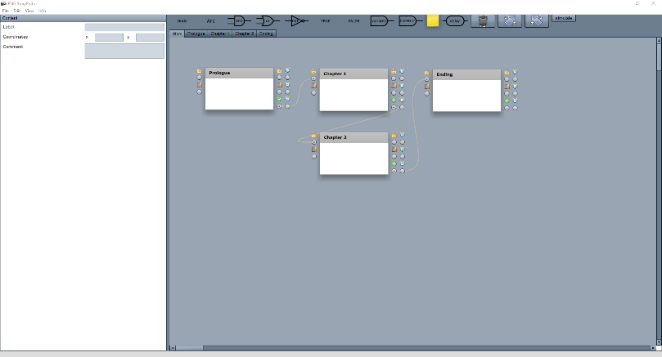
\includegraphics[width=\textwidth]{StoryEditor_SimpleStory}
        \caption{Story Editor interface}
        \label{fig:storyeditorinterface}
    \end{minipage}
    \hfill
    \begin{minipage}[b]{0.45\textwidth}
        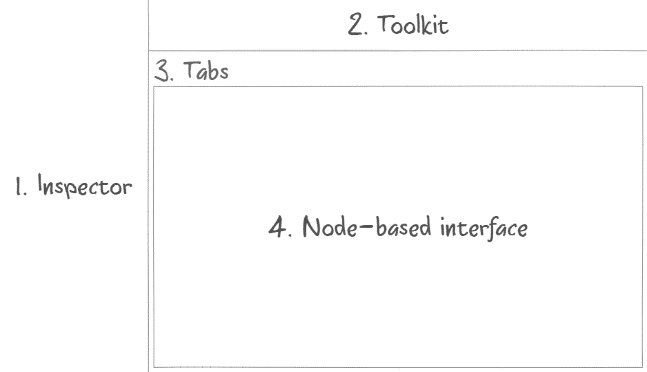
\includegraphics[width=\textwidth]{StoryEditor_ComponentWireFrame}
        \caption{Editor componenten}
        \label{fig:storyeditorcomponents}
    \end{minipage}
\end{figure}

Er bevindt zich een miniem aantal componenten op een enkele pagina. Dit duidt op de behoefte aan een kleine user interface library zonder navigatie functionaliteit.

% \begin{figure}[htb]
%     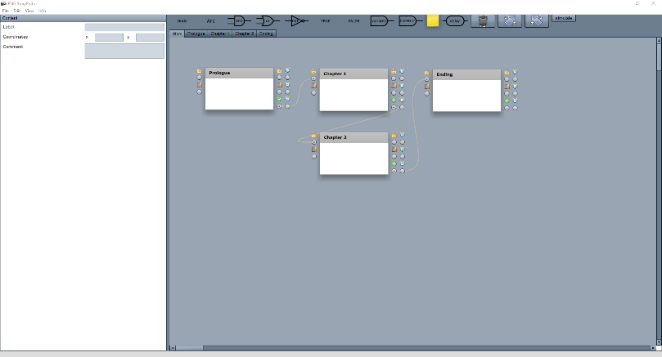
\includegraphics[width=\textwidth,height=\textheight,keepaspectratio]{StoryEditor_SimpleStory}
%     \caption{Story Editor interface}
%     \label{fig:storyeditorinterface}
%     \centering
% \end{figure}

% \begin{figure}[htb]
%     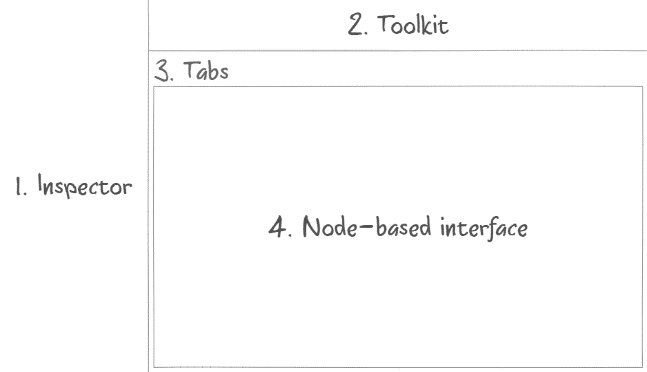
\includegraphics[width=\textwidth,height=\textheight,keepaspectratio]{StoryEditor_ComponentWireFrame}
%     \caption{Editor componenten}
%     \label{fig:storyeditorcomponents}
%     \centering
% \end{figure}

\clearpage
\subsection{User interface frameworks \& libraries}
Er zijn meerdere oplossingen beschikbaar voor het maken van user interfaces. Sommige bestaan uit een compleet raamwerk en een dwingen een bepaalde manier van werken af. Er kan gezegd worden dat deze een grote eigenzinnigheid hebben. Andere oplossingen zijn kleine libraries die zich alleen focussen op het inkapselen van componenten.

\subsubsection{Aandachtspunten}
Bij het zoeken naar een passende oplossing wordt er gekeken naar de volgende punten:
\begin{enumerate}
    \item De omvang van het ecosysteem
    \item Eigenzinnigheid
    \item Toekomstgerichtheid
    \begin{itemize}
        \item Wie onderhoudt/ steunt het project?
        \item Welke (populaire) producten gebruiken deze oplossing?
    \end{itemize}
    \item Snelheid
    \item Leercurve    
\end{enumerate}

\subsubsection{Verwachtingen}
Er wordt gezocht naar een oplossing waarmee componenten in gekapseld kunnen worden. Een ecosysteem met meerdere doeleinden kan worden beschouwd als overbodig. Zo bestaan de huidige editors uit één scherm wat een router\footnote{Een klasse die verantwoordelijk voor navigatie binnen een applicatie} overbodig maakt. Daarom zou een ecosysteem met een router redundant zijn.

Omdat er slechts gezocht wordt naar een component gebaseerde oplossing is het gewenst dat het raamwerk of de library vrijwel niet eigenzinnig is.

Verder is het belangrijk dat de ontwikkeling van het product actief is en dat deze niet snel zal verdwijnen. Een voorspelling kan gedaan worden op basis van (populaire) applicaties die het product gebruiken en of er (grote) bedrijven zijn die het product onderhouden of steunen.

Tenslotte zijn de snelheid en leercurve van het product minder belangrijk voor dit probleem, mits deze niet enorm afwijken van de rest. Bij de editor zal flexibiliteit en toekomstgerichtheid boven snelheid gaan. Hiernaast zal het ontwikkelen van een nieuwe editor moeten resulteren in een toekomstgerichte oplossing die nog voor jaren gebruik zal kunnen worden. Dit maakt het minder erg als de leercurve van het product iets hoger ligt.

\subsubsection{Selectie}
Om de staat van de applicatie synchroon te houden met de UI kan er gebruik worden gemaakt van bestaande oplossingen. Er is een selectie gemaakt uit populaire user interface raamwerken en libraries:
\begin{itemize}
    \item Vue
    \item Angular
    \item React
    \item Ember    
\end{itemize}

\pagebreak
\subsubsection{Resultaten}
De geselecteerde oplossingen zijn geanalyseerd op de eerdergenoemde aandachtspunten. Het resultaat wordt weergeven in \autoref{tab:uiframeworks}.

\begin{table}[htb]
    \centering
    \begin{tabular}{ l | p{2.5cm} p{2.5cm} p{2.5cm} p{2.5cm} }
    & \textbf{Vue}\footnote{https://vuejs.org/} & \textbf{Angular}\footnote{https://angular.io/} & \textbf{React}\footnote{https://reactjs.org/} & \textbf{Ember}\footnote{https://www.emberjs.com/}\\
    \hline
    \textbf{GitHub stats (05/03/2018)} & & &\\
    Volgers & 4.561 & 2.918 & 5.566 & 1.040\\
    Favorieten & 85.500 & 33.694 & 89.726 & 18.682\\
    Forks & 12.545 & 8.275 & 16.971 & 3.850\\
    \textbf{Gebacked door} & 1 persoon, Yuxi (Evan) You &Google & Facebook & LinkedIn, Netflix\\
    \textbf{"Native" language} & JavaScript & Typescript\footnote{TypeScript is een getypeerde ‘superset’ van JavaScript. Geschreven TypeScript code compileert naar JavaScript.} & JavaScript & JavaScript\\
    \textbf{TypeScript ondersteuning} & Ja, er zijn typing beschikbaar &Ja, out of the box & Ja, er zijn typing beschikbaar + typescript CLI\footnote{Command line interface tooling} & Ja, er zijn typing beschikbaar + typescript CLI\\
    \textbf{Ecosysteem} & Modulair, o.a. router, state management, cli, RxJS integration & Modulair, o.a. router, state management, cli, RxJS integration &	Modulair. Ecosysteem opgebouwd door community (e.g. community router) & Modulair, o.a. router, state management, cli\\
    \textbf{Leercurve} & \cellcolor{green!15}Makkelijk, door de flexibiliteit die Vue biedt & \cellcolor{red!25}Lastiger door de grote eigenzinnigheid dat het framework kent & \cellcolor{green!15}Makkelijk, het is een relatief kleine library & \cellcolor{red!25}Lastiger door de grote eigenzinnigheid dat het framework kent\\
    \textbf{Snelheid}\footnote{http://www.stefankrause.net/js-frameworks-benchmark7/table.html} & \cellcolor{green!15}Snel, Virtual DOM & \cellcolor{green!15}Snel & \cellcolor{green!15}Snel, Virtual DOM & \cellcolor{red!25}Langzaam\\
    \textbf{Eigenzinnigheid} & \cellcolor{green!15}Klein & \cellcolor{red!25}Groot, je moet in de kaders van angular werken & \cellcolor{green!15}Klein & \cellcolor{red!25}Groot\\
    \end{tabular}
    \caption[]{Inventarisatie van user interface frameworks en libraries \footnotemark}
    \label{tab:uiframeworks}
\end{table}
\footnotetext{Voor het laatst ingezien op: 05/03/2018}

\pagebreak
\subsubsection{Virtual DOM}
In het verleden waren webapplicaties statisch en relatief klein. Tegenwoordig wordt er veel gewerkt met (grotere) single page applications (SPA). Een SPA bestaat uit kleine individuele componenten die met elkaar kunnen communiceren en los van elkaar geüpdatet of vervangen kunnen worden\cite{SPA}. De webpagina wordt nooit in zijn geheel ververst of herladen. Hiernaast is een SPA verantwoordelijk voor het correct afhandelen van gebruikersinvoer.
Webapplicaties moet constant het document object model (DOM) achter de webpagina veranderen om feedback te kunnen tonen aan de gebruiker nadat deze input heeft geleverd. Voor grotere SPA-webapplicaties is dit een probleem, omdat DOM bestaat uit een boom. De nodes van de DOM boom zijn makkelijk af te gaan, maar in een grotere boom structuur (zoals in grote SPA applicaties) wordt dit al gauw een langdurig proces.
Hier komt virtual DOM in het spel. Dit is een abstractie van de ‘traditionele’ DOM\cite{Psaila2008}. Veranderingen in de virtual DOM resulteren in de executie van een verschil algoritme. Het resultaat van dit algoritme wordt vervolgens gereflecteerd in de “echte” DOM, waarin alleen de veranderde nodes aangepast worden. Door delen aan te passen in plaats van de gehele DOM kan de webapplicatie sneller reflecteren op de input van de gebruiker.
Zowel Vue als React maken gebruik van Virtual DOM.

\subsubsection{TypeScript}
Uit een onderzoek naar code kwaliteit op GitHub blijkt dat strongly typed programmeertalen minder gevoelig zijn voor fouten dan loosly typed programmeertalen\cite{Ray2014}. JavaScript is een voorbeeld van een loosly typed programmeertaal. Om code kwaliteit te verhogen en menselijke fouten te voorkomen wordt er geadviseerd om gebruik te maken van een strongly typed programmeertaal. Volgens onderzoek naar code kwaliteit op GitHub worden er minder fouten gemaakt in TypeScript projecten\cite{Ray2014}. TypeScript is een strongly typed superset van JavaScript, wat betekent dat TypeScript code gecompileerd kan worden naar JavaScript. Dit proces wordt ook wel transpiling genoemd.

TypeScript is ontwikkeld en wordt onderhouden door Microsoft. Hiernaast lijkt bijna iedere JavaScript library ondersteuning te bieden door typings aan te bieden. Typings zijn bestanden die TypeScript gebruikt om onderscheid te maken tussen verschillende types. Via deze typings kunnen JavaScript libraries samen werken met TypeScript code. 
Er is verder geen onderzoek gedaan naar alternatieven naast TypeScript, zo zou Flow\footnote{https://flow.org/} ook een oplossing kunnen zijn.

\subsection{Deel conclusie en aanbeveling}
Er wordt gezocht naar een kleine library die zich bezighoudt met het inkapselen van componenten. Alle vier de oplossingen beschikken over een modulair ecosysteem, maar React steekt hier bovenuit. React is een library wat betekend dat deze een relatief kleine omvang heeft in tegenstelling tot de andere oplossingen die gezien worden als frameworks. De oplossing van Facebook, React, regelt de synchronisatie tussen ingekapselde componenten en de staat van de applicatie.

Vue is een opkomende technologie die naast React ook een potentiele oplossing kan zijn. Net zoals React maakt Vue gebruik van virtual DOM, wat voor beide een positief effect op de snelheid waarmee componenten geüpdatet en vervangen worden. Hiernaast dwingen ze allebei geen strikte werkwijze af; ze kennen allebei een kleine eigenzinnigheid. Het ecosysteem van Vue biedt zelf meer “out of the box” functionaliteiten en heeft een bredere focus. Ondanks dat React zich alleen bezighoudt met het inkapselen van componenten heeft de community rondom React een eigen ecosysteem om React heen gebouwd.

Omdat er wordt gezocht naar een relatief kleine library die het mogelijk maakt om componenten te kunnen specificeren, is React in deze context een beter passende oplossing. React heeft een nauwe focus waar Vue een bredere focus heeft. Hiernaast wordt React gebruikt in producten van Facebook, Netflix\cite{NetflixReact} en in 2817+ andere tech stacks\footnote{https://stackshare.io/react/in-stacks}; de library heeft zichzelf bewezen. Vue is wat nieuwer en ondanks de toenemende populariteit wordt het minder gebruikt.

\section{Visual scripting interface}
Het doel van zowel de huidige als de nieuwe editor is om niet-programmeurs de game content aan te kunnen laten passen. Door gebruik te maken van een visual scripting interface kan de game content aangepast worden zonder enige programmeerkennis\cite{VisualScripting}. Stukken game content worden gezien als objecten met een visuele weergave die ook wel “nodes” genoemd worden. De eigenschappen van deze objecten kunnen vervolgens aanpast worden in de editor zelf.

Door nodes met elkaar te verbinden kan de gebruiker zonder een enkele lijn code het narratief moduleren.

\subsection{Diagramming libraries}
Visual scripting wordt toegepast op verschillende platformen\cite{UnityAssetStoreVisualScripting}\cite{NoFlo}\cite{GitHub3dVisualScripting}. Het wiel hoeft niet opnieuw uitgevonden te worden; bestaande oplossingen kunnen gebruikt worden voor het visualiseren van de nodes. Deze oplossingen gaan onder de naam ‘diagramming libraries’ omdat ze meestal gebruikt worden voor het tekenen van diagrammen. Er kan gebruik gemaakt worden van deze libraries om nodes te visualiseren.

\subsection{Eisen}
Voordat er een selectie aan libraries is gemaakt zijn er eisen opgesteld. Deze zijn gebaseerd op het MoSCoW principe. De eisen zijn verdeeld onder de volgende categorieën:

\begin{itemize}
    \item \textbf{M}ust have; randvoorwaarden en functionele eisen, vereist voor het product
    \item \textbf{S}hould have; operationele eisen met groot belang, behoeftes van het product
    \item \textbf{C}ould have; operationele eisen, behoeftes van het product
    \item \textbf{W}ould have; ontwerpbeperkingen, principes en (code)kwaliteitsbewaking
\end{itemize}

\subsubsection{Must have; de library moet}
\begin{itemize}
    \item Voorzien zijn van documentatie
    \item Restricties kunnen leggen op connecties tussen porten
    \item Nodes in elkaar kunnen voegen
    \item Nodes kunnen highlighten
    \item Controls (zoals input velden) op nodes kunnen leggen
\end{itemize}

\subsubsection{Should have; het is van belang dat de library}
\begin{itemize}
    \item Nodes kunnen copy/ pasten*
    \item Acties ongedaan kunnen maken*
    \item Een navigeerbaar canvas aanbieden**
    \item Group selectie mogelijk maakt*
    \item De mogelijkheid biedt om grafen in grafen in te kunnen maken (sub-graphs).
\end{itemize}

\subsubsection{Could have; het is mooi meegenomen als de library}
\begin{itemize}
    \item Een minimap kan tonen waarop alle nodes zichtbaar zijn
    \item Real-time collaboratie toelaat
    \item De nodes kan ordenen
    \item De nodes snapt op een raster
    \item Een zoekfunctie biedt
    \item Een verschil algoritme implementeert
    \item Het groeperen van nodes mogelijk maakt
\end{itemize}

\subsubsection{Would have; om de houdbaarheid van het product te verhogen moeten de library}
\begin{itemize}
    \item Typings aanbieden
\end{itemize}

\noindent \textit{* zou eventueel zelf met relatief weinig moeite geïmplementeerd kunnen worden}\\
\textit{** er kan gebruik gemaakt worden van andere oplossingen voor dit probleem}\footnote{https://github.com/ariutta/svg-pan-zoom}

\subsubsection{Selectie en analyse}
Er is een selectie gemaakt uit JavaScript diagramming libraries:
\begin{itemize}
    \item D3-node-editor\footnote{https://github.com/Ni55aN/d3-node-editor}
    \item wcPlay\footnote{https://github.com/WebCabin/wcPlay}
    \item JointJS\footnote{ https://github.com/clientIO/joint}
    \item JointJS + Rappid (commerciële versie van JointJS)\footnote{https://www.jointjs.com/}
    \item MxGraph\footnote{https://github.com/jgraph/mxgraph}
    \item GoJS\footnote{https://gojs.net/latest/index.html}
\end{itemize}

\noindent De selectie aan diagramming libraries is afgezet tegen de opgestelde eisen en op genomen in \autoref{tab:diagramminglibraryfunctionality}.

\begin{landscape}
    \begin{figure}[H]
        % 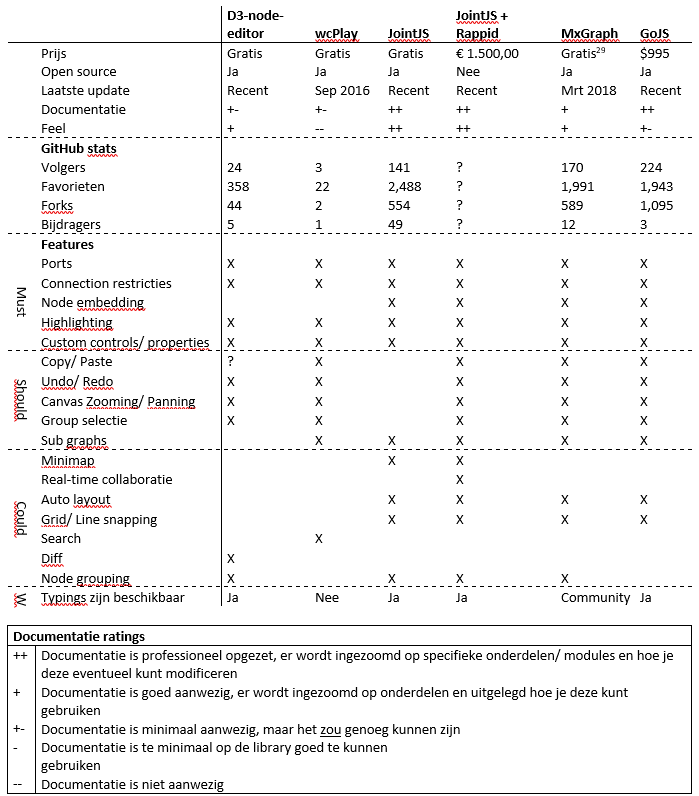
\includegraphics[width=\textwidth]{DiagrammingLibraryMatrix}
        \centering
        \resizebox{.8\columnwidth}{!}{
            \begin{tabular}{ l l | l l l l l l }
                \ & \ & \textbf{D3-node-editor} & \textbf{wcPlay} & \textbf{JointJS} & \textbf{JointJS + Rappid} & \textbf{MxGraph} & \textbf{GoJS}\\ \hline
                & Prijs & Gratis & Gratis & Gratis & \euro 1500 & Gratis & \euro 995 \\
                & Open source & Ja & Ja & Ja & Nee & Ja & Ja  \\ 
                & Laatste update & Recent & Sep 2016 & Recent & Recent & 01/03/2018 & Recent  \\
                & Documentatie & +-- & +-- & ++ & ++ & + & ++  \\
                & Feel & + & -- -- & ++ & ++ & + & +-- \\ \hdashline
                & \textbf{GitHub stats (16/05/2018)} &  &  &  &  &  &  \\ 
                & Volgers & 24 & 3 & 141 & - & 170 & 224 \\
                & Favorieten & 358 & 22 & 2.488 & - & 1.991 & 1.943 \\
                & Forks & 44 & 2 & 554 & - & 589 & 1.095 \\
                & Bijdragers & 5 & 1 & 49 & - & 12 & 3 \\ \hdashline
                & \textbf{Features} &  &  &  &  &  & \\
                \multirow{5}{*}{Must} & Ports & X & X & X & X & X & X \\ 
                & Connection restricties & X & X & X & X & X & X \\
                & Node embedding &  &  & X & X & X & X \\
                & Highlighting & X & X & X & X & X & X \\
                & Custom controls/ properties & X & X & X & X & X & X \\ \hdashline
                \multirow{5}{*}{Should} & Copy/ Paste & ? & X &  & X & X & X \\
                & Undo/ Redo & X & X &  & X & X & X \\
                & Canvas Zooming/ Panning & X & X &  & X & X & X \\
                & Group selectie & X & X &  & X & X & X \\
                & Sub graphs &  & X & X & X & X & X \\ \hdashline
                \multirow{6}{*}{Could} & Minimap &  &  & X & X &  &  \\
                & Real-time collaboratie &  &  &  & X &  &  \\
                & Auto layout &  &  & X & X & X & X \\
                & Grid/ Line snapping &  &  & X & X & X & X \\
                & Search &  & X &  &  &  &  \\
                & Diff & X &  &  &  &  &  \\
                & Node grouping & X &  & X & X & X &  \\ \hdashline
                \multirow{1}{*}{Would} & Typings zijn beschikbaar & Ja & Nee & Ja & Ja & Community & Ja \\
            \end{tabular}
        }
            
        \caption[]{Diagramming libraries en hun functionaliteiten \footnotemark}
        \label{tab:diagramminglibraryfunctionality}
    \end{figure}
    \footnotetext{Voor het laatst ingezien op: 16/05/2018}
\end{landscape}

\subsection{Deel conclusie en aanbevelingen}
Uit de analyse blijkt dat ‘D3-node-editor’ en ‘wcPlay’ niet voldoen aan de randvoorwaarden. Dit lag vooral aan de matige documentatie die de libraries meeleveren. Hierdoor is het erg lastig om de libraries toe te passen.

MxGraph en Rappid beschikken beide over een grote feature set die voldoen aan de requirements die vooraf opgesteld zijn. MxGraph was voorheen een commerciële oplossing, maar is nu gratis te gebruiken. Rappid met JointJS is de betaalde optie met collaborative editing functionaliteit. Hiernaast lijkt de community rondom JointJS groter; de library lijkt populairder te zijn dan MxGraph.

De commerciële optie, Rappid met JointJS, komt met betere documentatie en mogelijke ondersteuning. Dit kan essentieel zijn bij het opzetten van de editors. De collaborative editing functionaliteit van Rappid zou eventueel ook interessant kunnen zijn voor het bedrijf.

In het prototype is er gekozen voor de optie die voldoet aan de meeste eisen: JointJS + Rappid. Daarentegen is Rappid betaald en er zal daarom in het prototype gewerkt worden met JointJS. Deze voldoet aan de randvoorwaarden en biedt genoeg functionaliteit om het prototype te ondersteunen. Rappid is een laag bovenop JointJS en zou eventueel later toegevoegd kunnen worden.

\section{Conclusie}
Met dit hoofdstuk wordt de volgende deelvraag beantwoord: “Hoe kan er een ‘technology stack’ opgezet worden die een flexibele basis biedt voor een editor waarmee diverse digitale interactieve verhalen verteld kunnen worden?”.

Electron biedt een battle tested platform dat wordt onderhouden door GitHub. Door gebruik te maken van Electron als ontwikkelplatform kunnen desktopapplicaties worden ontwikkeld met behulp van webtechnologieën. Rondom webtechnologieën bevindt zich een grote community die oplossingen voor bestaande problemen realiseert. Daarnaast kan code hergebruikt worden wanneer deze wordt verplaatst naar een webomgeving. Het kunnen kiezen uit bestaande oplossingen en hergebruiken van code wanneer de editor gemigreerd wordt naar een webomgeving brengt veel flexibiliteit met zich mee.

Om de user interface (UI) synchroon te houden met de staat van de applicatie is er gekozen voor de React library die onderhouden wordt door Facebook. Deze library focust zich op het inkapselen van UI-componenten en helpt bij het houdbaar en flexibel opzetten van de editor UI.

De web development community biedt vele oplossingen op visual scripting interfaces. Deze diagramming libraries nemen veel werk uit handen bij het opzetten van de nieuwe editors. JointJS en Rappid worden aangeraden als diagramming library vanwege de documentatie, eventuele ondersteuning en collaborative editing functionaliteit.

Het voorstel voor de nieuwe technology stack van \&ranj wordt weergeven in \autoref{tab:newtechstack}. Hierin zijn veranderingen aangegeven in orange. Er wordt weg gestapt van Apache Flex en haar onzekere toekomst. Door weg te stappen van Apache Flex komt de verouderde AS3 software library te vervallen waardoor er nog maar één software library onderhouden hoeft te worden. Rappid beschikt over duidelijke documentatie en collaborative editing functionaliteiten, waarvan \&ranj in de toekomst gebruik van kan maken. Tenslotte kan er code hergebruikt worden wanneer er gemigreerd wordt naar een webomgeving, omdat het geheel geschreven is met behulp van webtechnologieën.

\begin{table}[htb]
    \centering
    \begin{tabular}{ | l | l | }
        \hline
        \multicolumn{2}{|c|}{\textbf{Narrative game - Technology stack}} \\
        \hline
        \multicolumn{2}{|c|}{Application and Data} \\
        \hline
        \&ranj JavaScript software library & \tabitem Javascript(ECMAScript5) \\
        & \tabitem CreateJS suite \\
        \hline
        Narrative game template & \tabitem Javascript(ECMAScript5) \\
        & \tabitem CreateJS suite \\
        & \tabitem SomaJS \\
        \hline            
        \cellcolor{orange!15}Editor(s) & \cellcolor{orange!15}\tabitem Electron \\
        \cellcolor{orange!15}& \cellcolor{orange!15}\tabitem React \\
        \cellcolor{orange!15}& \cellcolor{orange!15}\tabitem TypeScript \\
        \cellcolor{orange!15}& \cellcolor{orange!15}\tabitem JointJS + Rappid \\
        \hline
        \multicolumn{2}{|c|}{Utilities} \\
        \hline
        Analytics & \tabitem Google Analytics \\
        \hline
        \multicolumn{2}{|c|}{DevOps} \\
        \hline
        Source control & \tabitem Beanstalk \\
        & \tabitem SourceTree \\
        \hline
        Deployment & \tabitem Jenkins \\
        & \tabitem SourceTree \\
        \hline
        \cellcolor{orange!15}IDE'S & \cellcolor{orange!15}\tabitem Netbeans \\
        \hline
        Monitoring & \tabitem Pingdom \\
        \hline
        \multicolumn{2}{|c|}{Business Tools} \\
        \hline
        Collaboratie & \tabitem Trello \\
        & \tabitem G Suite \\        
        & \tabitem Slack \\
        \hline
        Documentatie & \tabitem \&ranj wiki \\
        \hline
    \end{tabular}
    \caption{Voorstel op de nieuwe technology stack}
    \label{tab:newtechstack}
\end{table}